
\documentclass[11pt]{article}

\usepackage[margin=1in]{geometry}
\usepackage{graphicx}
\usepackage{booktabs}
\usepackage{hyperref}

\title{QBS 103 Final Project}
\author{Pinzhang Zhu}
\date{November 9, 2026}

\begin{document}

\maketitle

\section{Methods}
\subsection{Data Source and Preparation}

This project used gene expression and maternal characteristic data from the Vitamin D Antenatal Asthma Reduction Trial (VDAART), described in the original study \cite{mirzakhani_early_2016}. The GSE85307 dataset included 157 samples: 110 from normal pregnancies and 47 from pregnancies with preeclampsia.

Gene expression data were matched with maternal characteristics using GEO sample IDs. Text prefixes were removed from the covariate values, and continuous variables were converted to numeric format. Maternal BMI was divided into two categories using a cutoff of 25 kg/m$^2$. All 157 samples were retained in the analysis.

\subsection{Data Analysis and Visualization}

Maternal age, gestational age at delivery, and maternal vitamin D levels were summarized using means and standard deviations. Pregnancy outcome and BMI category were summarized using counts and percentages.

Histograms, scatterplots, and boxplots were created for three genes: \textit{PTX3}, \textit{ABCA9}, and \textit{ACTG2}. Scatterplots included fitted linear trends, while boxplots displayed individual observations.

The heatmap included these three genes and seven additional genes from the available gene list. Expression values were standardized within each gene. Hierarchical clustering was applied to both genes and samples, with tracking bars for pregnancy outcome and maternal BMI category.

An alluvial plot was used to visualize the distribution of samples across the two categorical variables. No formal hypothesis tests were performed.

\subsection{Software}

All analyses were conducted using R version 4.5.1
\cite{r_core_team_r_2025}.

Data processing and visualization used tidyverse
(version 2.0.0) \cite{wickham_welcome_2019},
ggplot2 (version 4.0.2) \cite{wickham_ggplot2_2016},
and ggpubr (version 1.0.0)
\cite{kassambara_ggpubr_2026}.

Heatmaps were generated using pheatmap
(version 1.0.13) \cite{kolde_pheatmap_2025},
and alluvial plots were created using ggalluvial
(version 0.12.6) \cite{brunson_ggalluvial_2020}.

The report was generated from R Markdown using
knitr (version 1.52) \cite{yihui_xie_knitr_2026}.

The complete project code is available at
\url{https://github.com/zhualtis-gif/HSE103_FinalProject}.

\section{Results}

\subsection{Maternal Characteristics}

The dataset included 157 samples, including 110 normal pregnancies and 47 pregnancies with preeclampsia.

Maternal age was similar between the two groups. Compared with the normal pregnancy group, the preeclampsia group had a lower mean gestational age at delivery (37.8 vs. 39.3 weeks) and a lower mean maternal vitamin D level (19.7 vs. 24.4 ng/mL).

The proportion of mothers with BMI $\geq 25$ was higher in the preeclampsia group (72.3\% vs. 63.6\%) (Table~\ref{tab:characteristics}).


\begin{table}[htbp]
\centering

\caption{Maternal characteristics by pregnancy outcome}
\label{tab:characteristics}

\begin{tabular}{lcc}
\toprule
Characteristic & Normal (n = 110) & Preeclampsia (n = 47) \\
\midrule
Maternal age (years) & 26.6 (5.1) & 25.8 (4.9) \\
Gestational age at delivery (weeks) & 39.3 (1.0) & 37.8 (3.5) \\
Maternal vitamin D (ng/mL) & 24.4 (14.5) & 19.7 (8.3) \\
BMI below 25 & 40 (36.4\%) & 13 (27.7\%) \\
BMI 25 or higher & 70 (63.6\%) & 34 (72.3\%) \\
\bottomrule
\end{tabular}

\par\smallskip
{\small Continuous variables are presented as mean (SD);
categorical variables as n (\%).}

\end{table}


\subsection{Gene Expression Distributions}

The expression distributions differed across the three
selected genes. \textit{PTX3} showed a slightly right-skewed
distribution, while \textit{ABCA9} expression values were
more concentrated. Most \textit{ACTG2} expression values
were within a narrow range, with a few notably high
observations (Figure~\ref{fig:histograms}).

\begin{figure}[htbp]
\centering

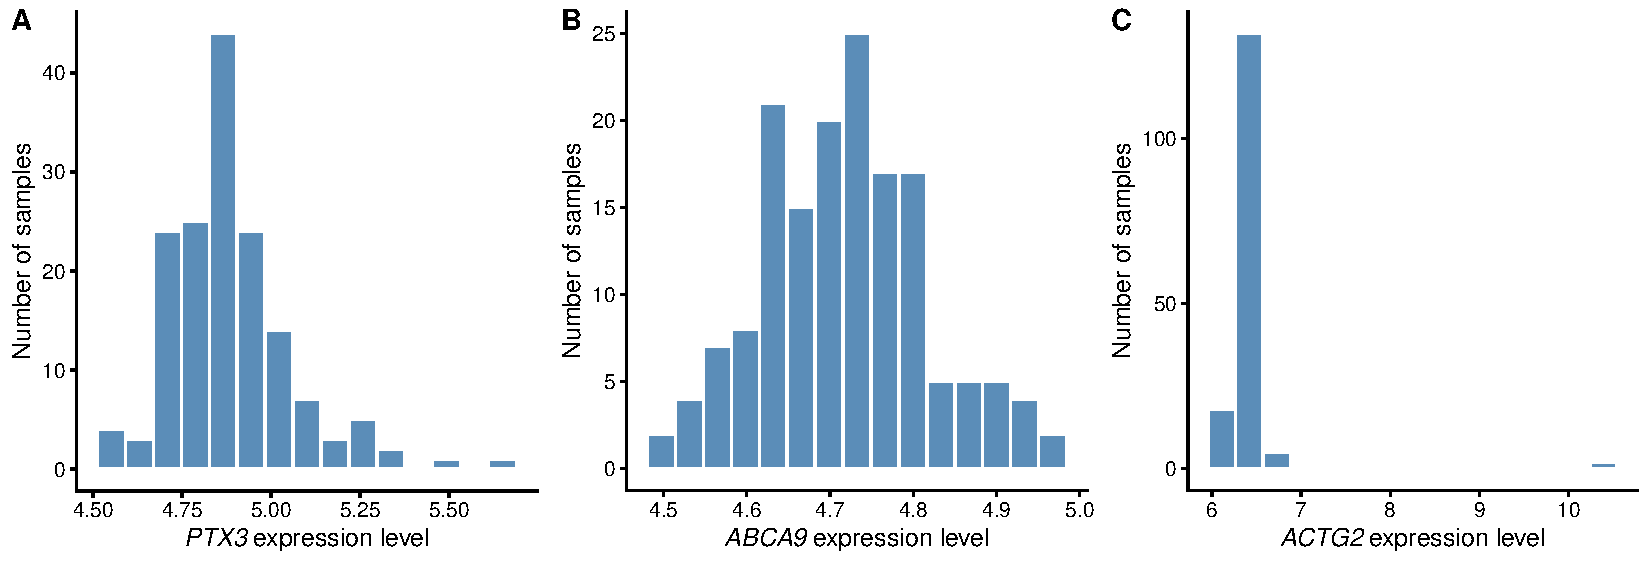
\includegraphics[width=\textwidth]{figure1.pdf}

\caption{Gene expression distributions across 157 samples:
(A) \textit{PTX3}, (B) \textit{ABCA9}, and
(C) \textit{ACTG2}. Each histogram shows the number of
samples within each expression interval.}

\label{fig:histograms}
\end{figure}

\subsection{Maternal Age and Gene Expression}

The scatterplots showed weak linear trends between
maternal age and expression levels for all three genes.
No clear linear relationship was visible for
\textit{PTX3}, \textit{ABCA9}, or \textit{ACTG2}
(Figure~\ref{fig:scatterplots}).

\begin{figure}[htbp]
\centering
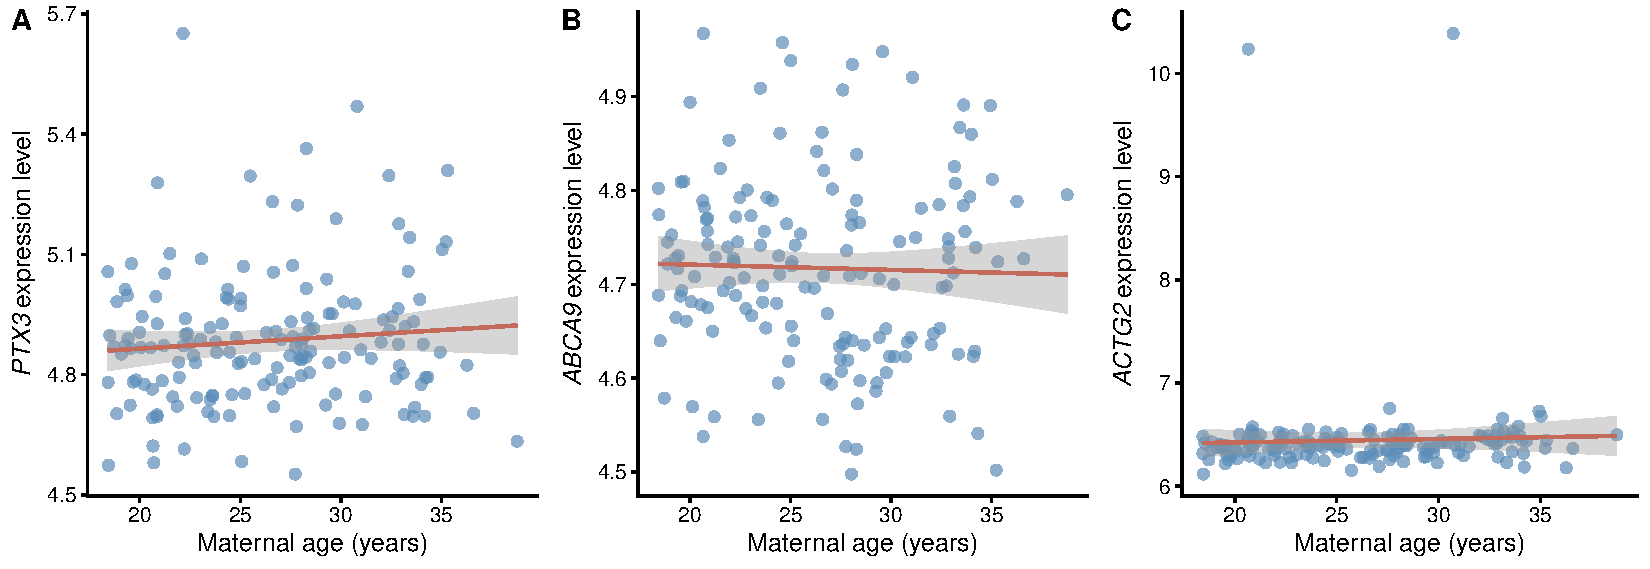
\includegraphics[width=\textwidth]{figure2.pdf}
\caption{Gene expression levels in relation to maternal age:
(A) \textit{PTX3}, (B) \textit{ABCA9}, and
(C) \textit{ACTG2}. Each point represents one sample.
The fitted lines show linear trends, with shaded areas
indicating 95\% confidence intervals.}
\label{fig:scatterplots}
\end{figure}

\subsection{Gene Expression by Pregnancy Outcome and BMI}

Gene expression distributions overlapped across pregnancy
outcome and BMI groups. Some differences in group medians
were visible for \textit{ABCA9}, while \textit{PTX3}
and \textit{ACTG2} showed relatively similar expression
levels across the groups (Figure~\ref{fig:boxplots}).

\begin{figure}[htbp]
\centering
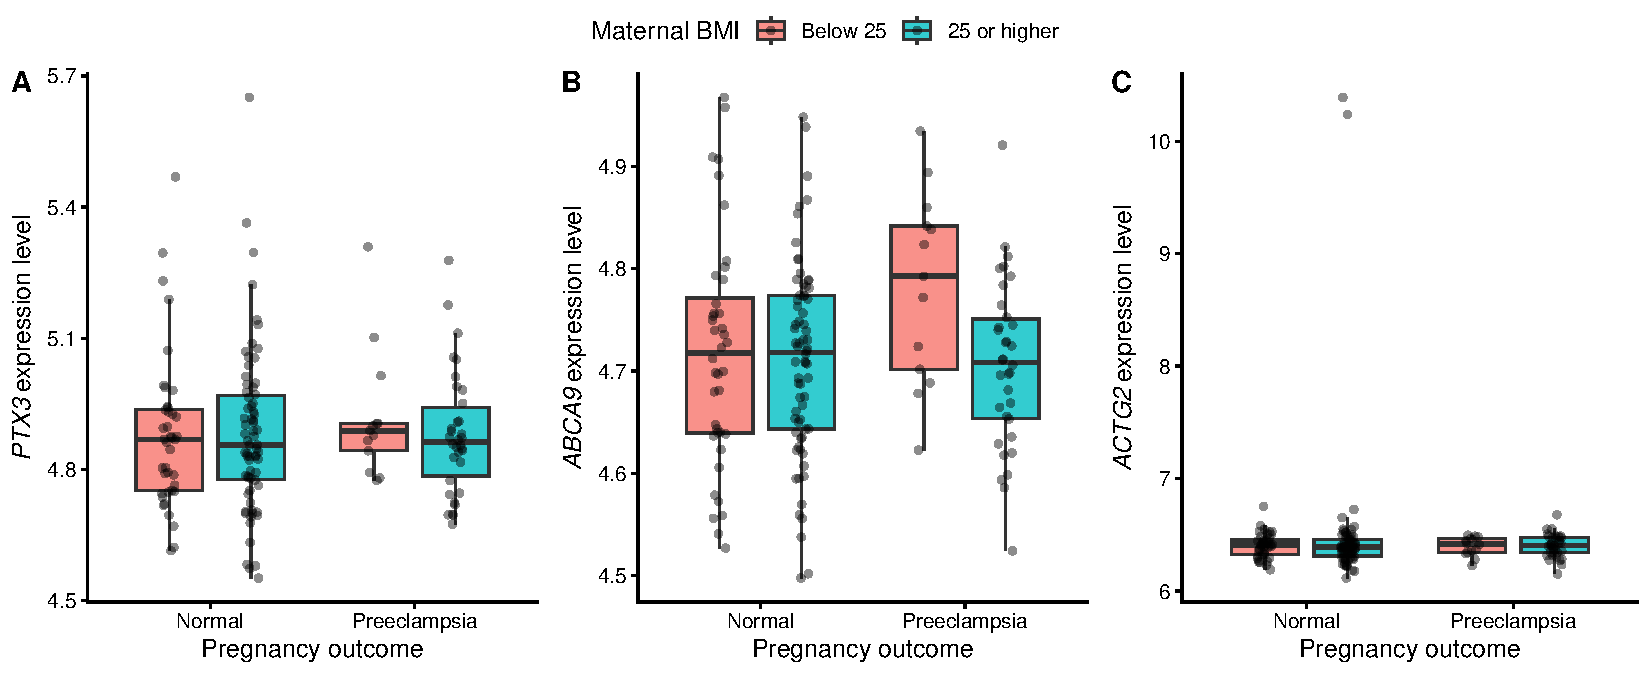
\includegraphics[width=\textwidth]{figure3.pdf}
\caption{Gene expression by pregnancy outcome and
maternal BMI category: (A) \textit{PTX3},
(B) \textit{ABCA9}, and (C) \textit{ACTG2}.
Boxes show the median and interquartile range,
while jittered points represent individual samples.}
\label{fig:boxplots}
\end{figure}


\subsection{Gene Expression Heatmap}

Figure~\ref{fig:heatmap} shows the expression patterns of
ten selected genes across 157 samples. Expression levels
varied across samples, with a few notably high values.
The clustering did not show a clear separation between
normal and preeclampsia samples.

\begin{figure}[htbp]
\centering
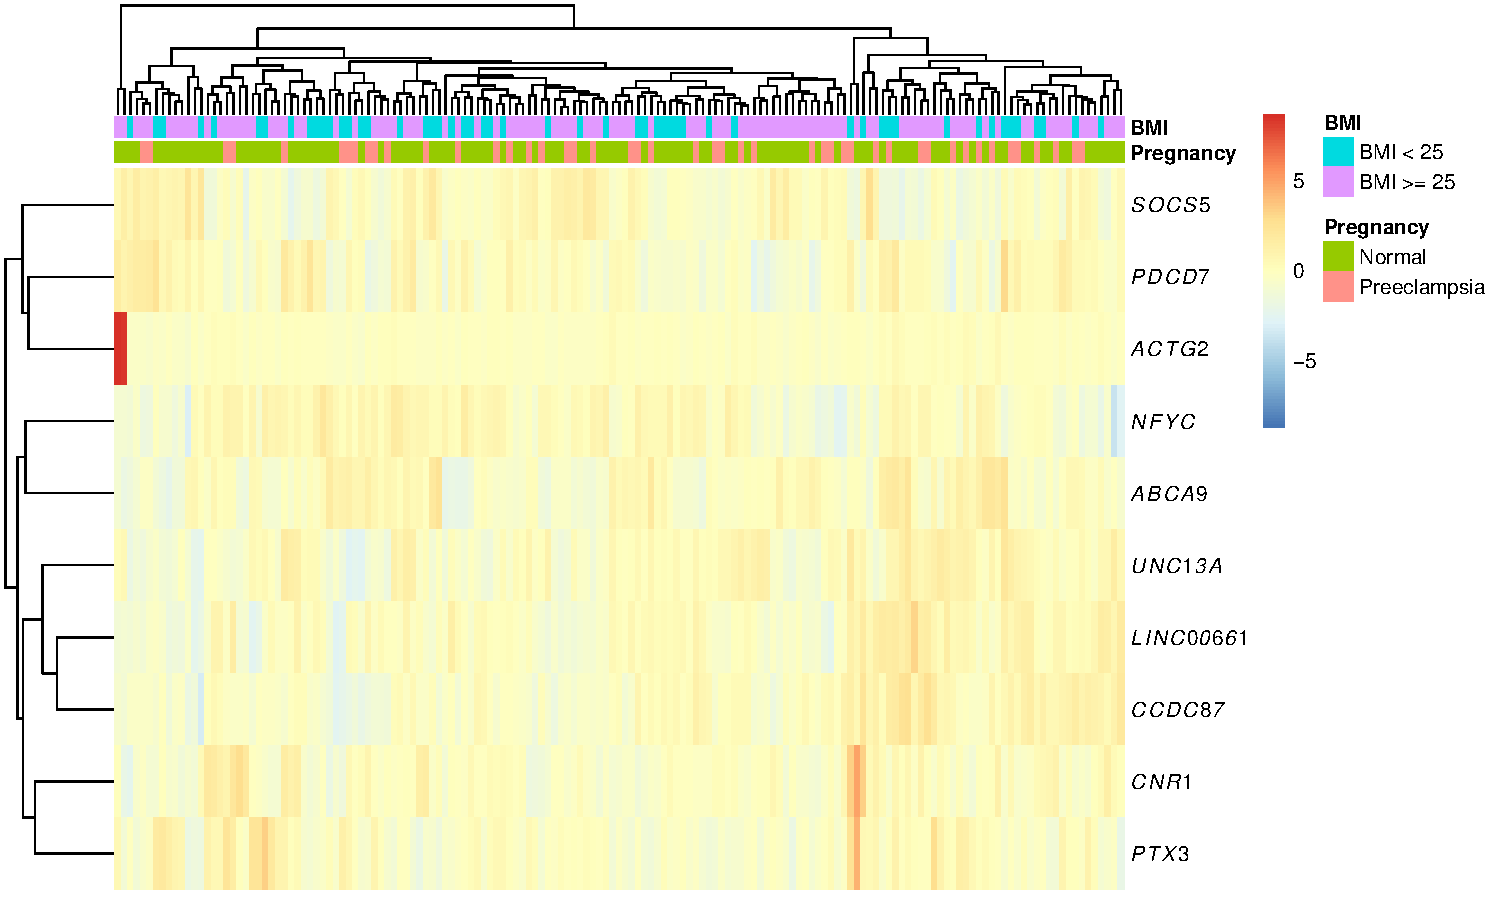
\includegraphics[width=\textwidth]{figure4.pdf}
\caption{Heatmap of ten selected genes across 157 samples.
Expression values were standardized within each gene.
Hierarchical clustering was applied to genes and samples.
The tracking bars indicate pregnancy outcome and maternal
BMI category.}
\label{fig:heatmap}
\end{figure}


\subsection{Maternal BMI and Pregnancy Outcome}

Figure~\ref{fig:alluvial} illustrates the distribution
of maternal BMI categories across pregnancy outcomes.
Among 157 samples, 53 mothers had a BMI below 25 and
104 had a BMI of 25 or higher. The flows show the
number of normal and preeclampsia pregnancies within
each BMI category.

\begin{figure}[htbp]
\centering
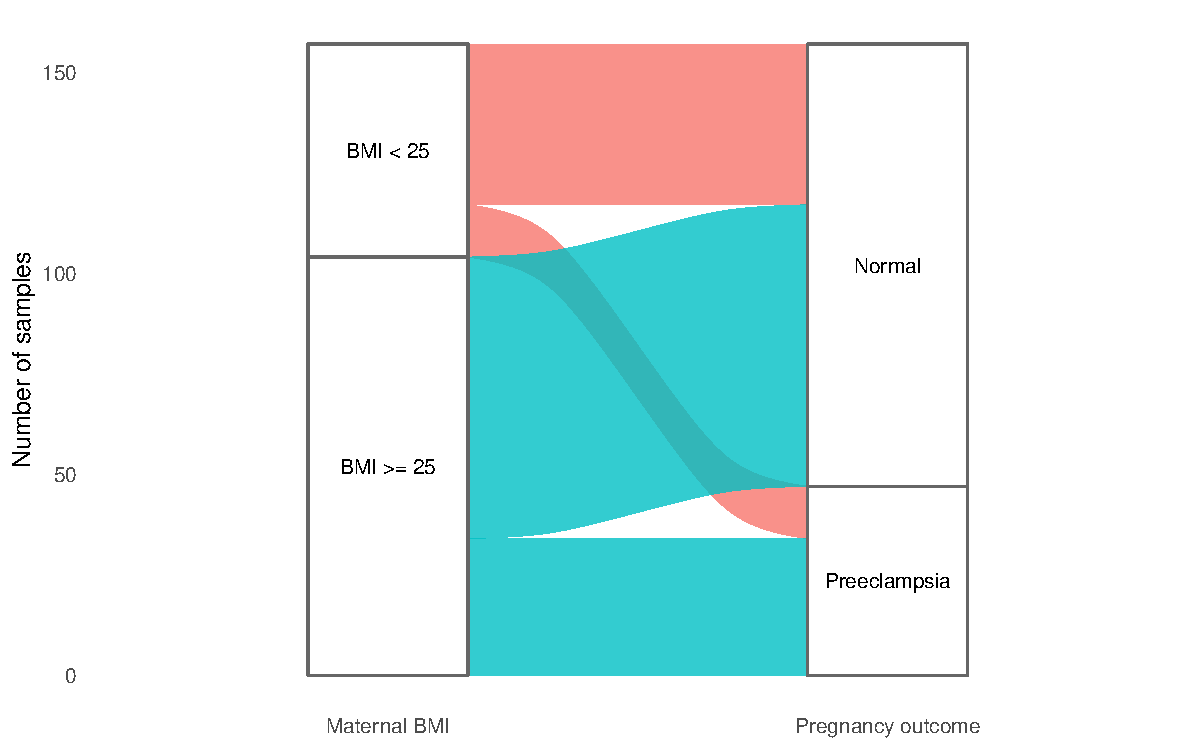
\includegraphics[width=0.85\textwidth]{figure5.pdf}
\caption{Alluvial plot showing the distribution of
maternal BMI categories across normal and preeclampsia
pregnancies. The width of each flow represents the
number of samples in that group.}
\label{fig:alluvial}
\end{figure}

\bibliographystyle{plain}
\bibliography{references}

\end{document}
